\clearpage
\section{Auswertung}
\subsection{Bestimmung der zeitlichen Verzögerungen}
Da hauptsächlich der NaJ-Szintillationszähler verwendet wird, wurden für diesen die zeitlichen Verzögerungen der Elektronik bestimmt. Diese wurden mithilfe der Diagramme, welche die jeweiligen Signale anzeigen, abgelesen (s. Anhang). \\
Die Verzögerung ist die zeitliche Differenz zwischen dem Einsatz der beiden Signale.\\
\subsubsection{Plastik-Szintillator}
Das Signal des Plastik-Szintillators wurde ohne Verstärkung bei einer Spannung von $U_{Plastik}=(1900\pm2)V$ vermessen. Das Signal hat eine periodische Form mit mehreren Peaks, wodurch die Verarbeitung und Auswertung des Signals erschwert wird. Dies ist auch der Grund, weshalb vornehmlich der NaJ-Szintillator verwendet wird.
\subsubsection{Verzögerung zwischen dem Amplifier-Eingang und dem unipolaren Ausgang}
Diese Verzögerung lasen wir zu $\Delta t=(3,7\pm0,5)\mu s$ ab. Der Fehler ergibt sich dabei durch die Ableseungenauigkeit.
\subsubsection{Verzögerung zwischen dem Amplifier-Eingang und dem bipolaren Ausgang}
Diese Verzögerung wurde zu $\Delta t=(1,5\pm0,5)\mu s$ bestimmt.
\subsubsection{Verzögerung zwischen dem Amplifier-Eingang und dem Ausgang des SCA}
Hierbei war eine Shaping Time von $3 \mu s$ eingestellt. Die Verzögerung wurde dann zu $\Delta t=(8,0\pm0,5)\mu s$ abgelesen. Bei Variierung der Shaping Time fiel auf, dass die Zeitdifferenz zwischen dem Ausgangssignal des Amplifier-Eingangs und dem Ausgang des SCA proportional zur Shaping Time ist. Dies bestätigt die Erwartung, da die Shaping Time eine Integrationsdauer angibt, über welche das Signal aufintegriert wird. \\
Bei den Ergebnissen handelt es sich natürlich nur um ungefähre Werte, deren Genauigkeit für eine qualitative Betrachtung allerdings ausreichend ist.
\clearpage
\subsection{Betrachtung des Untergrunds}
In den folgenden Schritten wurde jeweils der NaJ-Szintillationszähler verwendet. Da für diese eine Untergrundkorrektur benötigt wird, wurde für jeden Kanal des MCA die Zählrate $n_{u}=\frac{Counts~N}{Live~time~t}$ bestimmt. Dabei wurde statt der voreingestellten 'Real time' die 'Live time' verwendet, da diese die Dauer angibt, in welcher nicht gerade Pulse verarbeitet wurden und die Software somit unempfänglich für Counts war. Für die Untergrundmessung betrug die 'Live time' $t=32333 s$.\\
 Der Fehler der Counts berechnet sich, wenn man den Fehler auf die Zeit vernachlässigt, mithilfe der Gauss'schen Fehlerfortpflanzung zu $s_{n_{u}}=\frac{\sqrt{N}}{t}$, da N poissonverteilt ist und deswegen $s_{N}=\sqrt{N}$ gilt. \\
 Das Diagramm der über die Kanäle aufgetragenen Raten sieht folgendermaßen aus:
 \begin{figure}[h]
 \begin{center}
 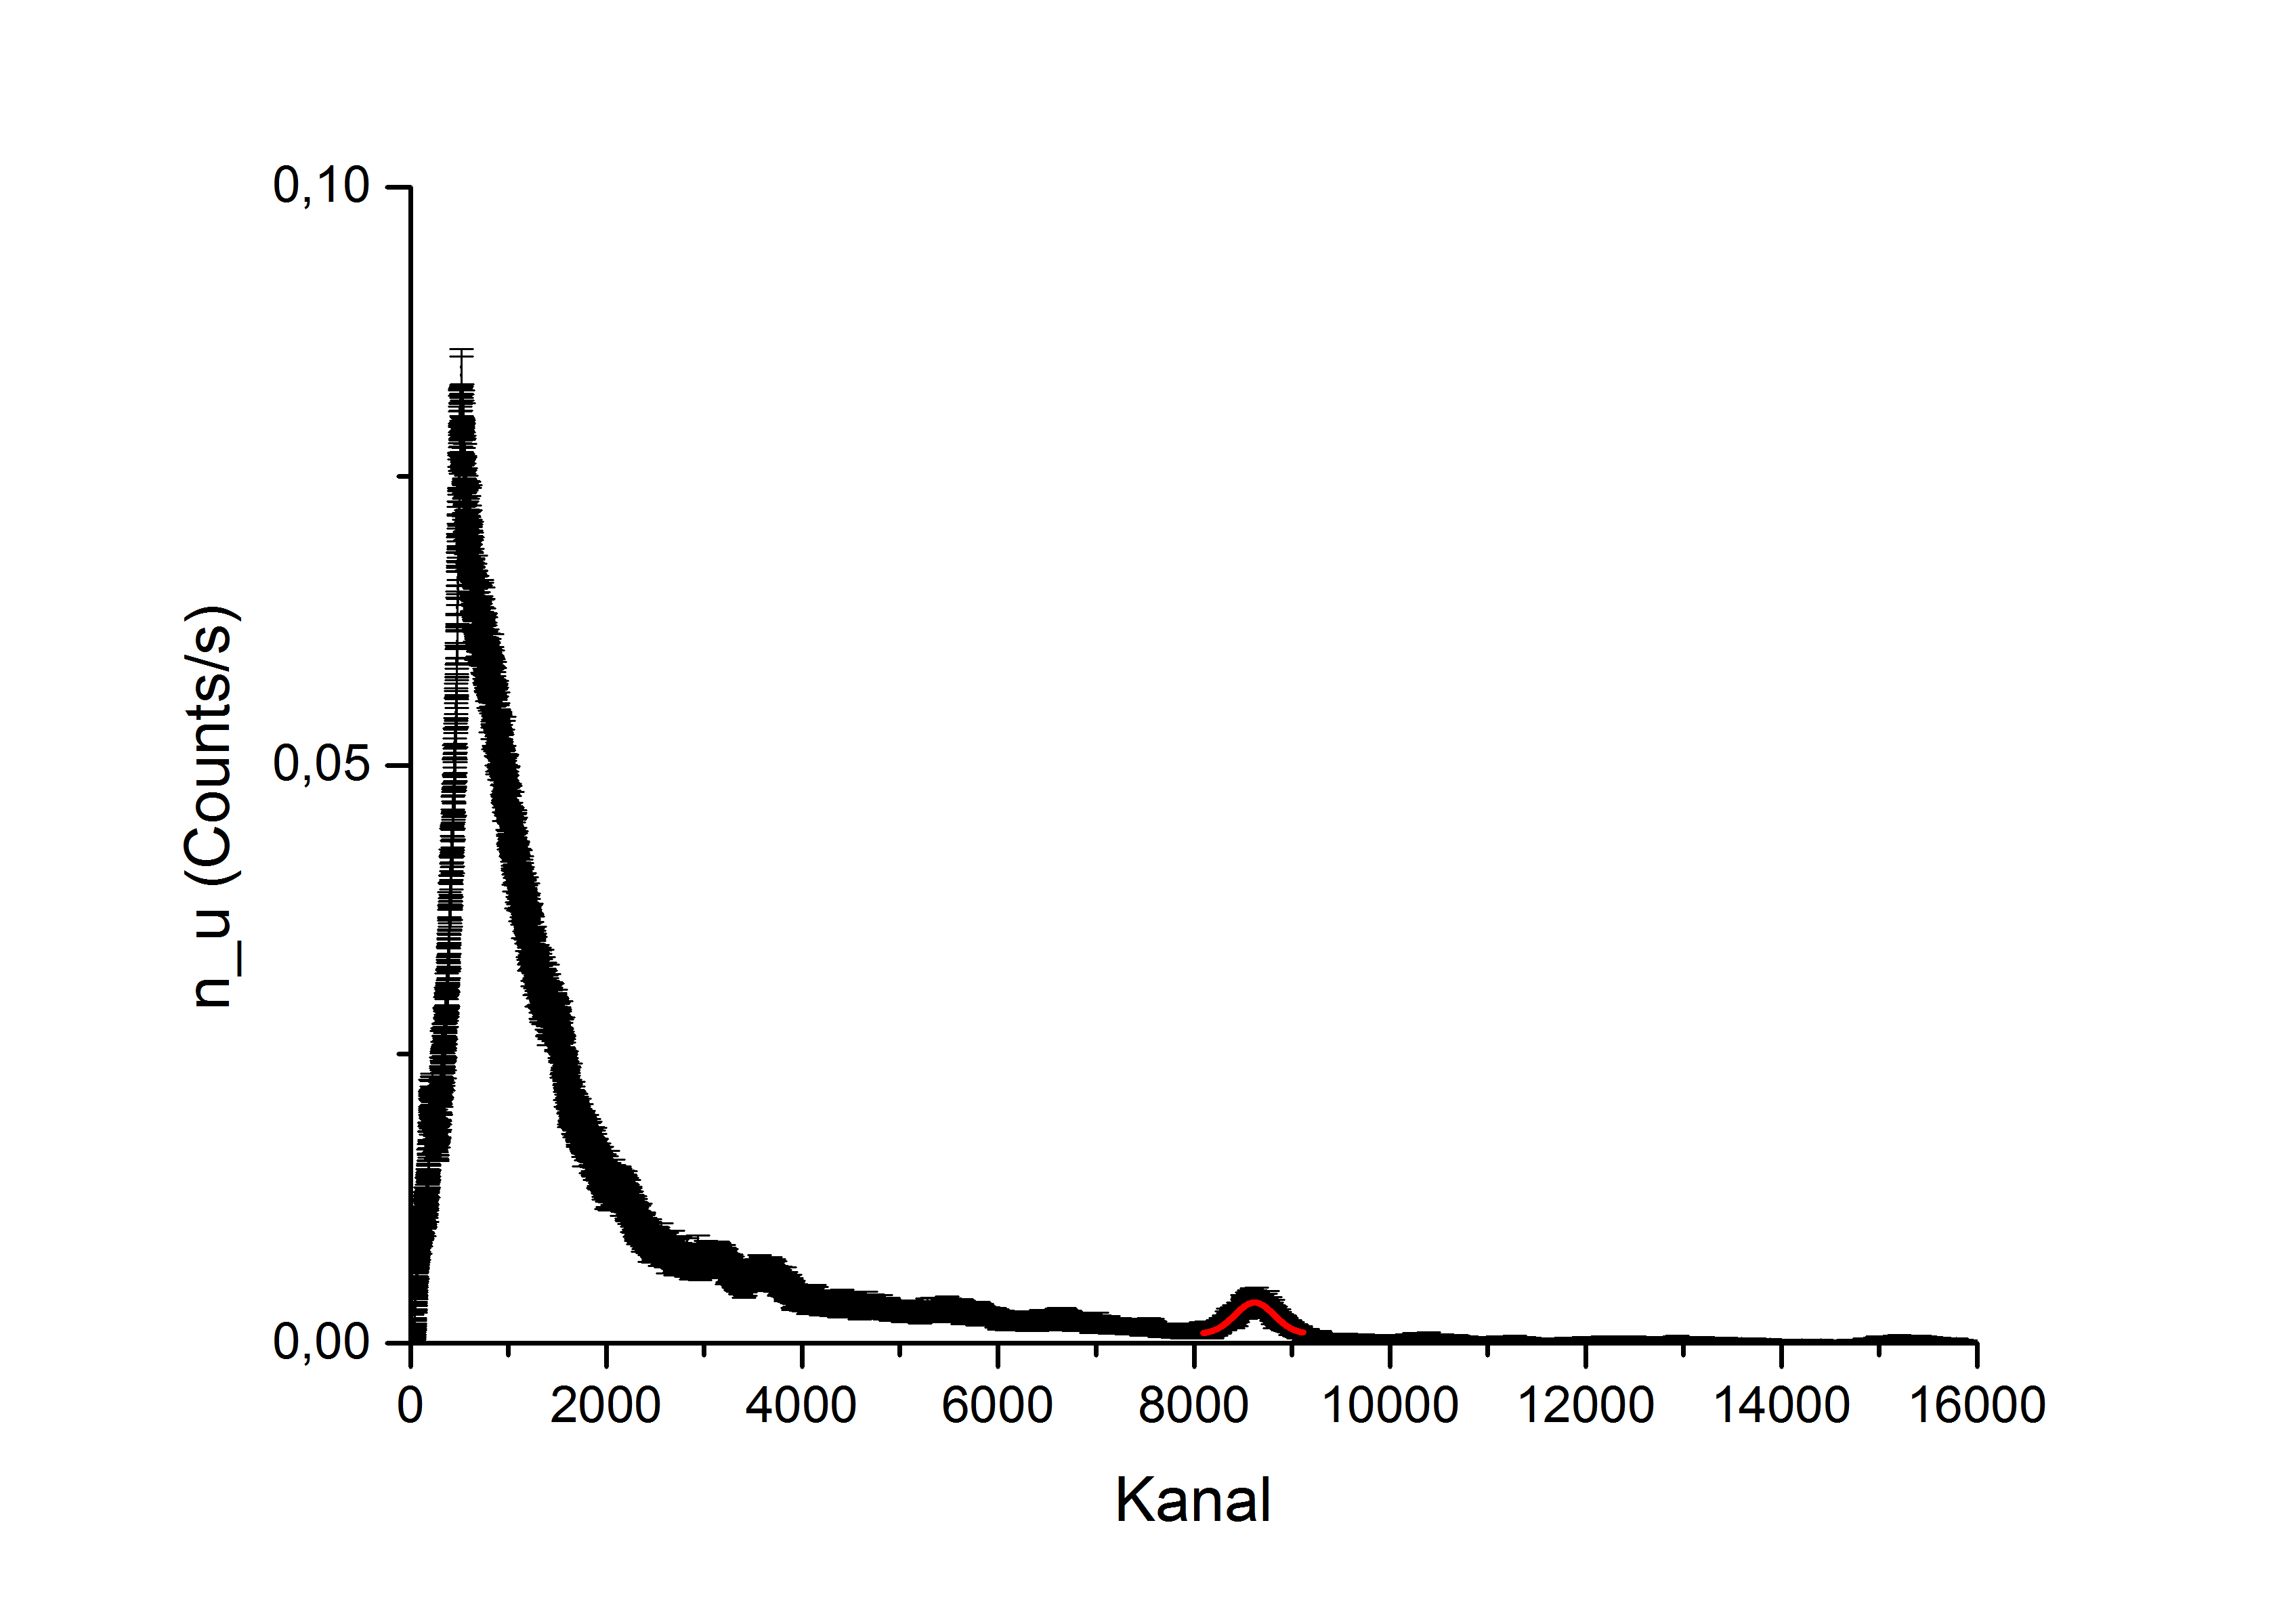
\includegraphics[scale=0.6]{Bilder/ugrund}
 \caption{Untergrundzählraten}
 \end{center}
 \end{figure}
 ~\\
 Dabei ist bei Kanal klar ein Peak zu erkennen, auf welchen wir später, nach der Energieeichung, noch zurückkommen werden.
 \subsection{Energieeichung}
 Um eine Energieeichung durchführen zu können, wurden die Spektren von $^{22}Na$, $^{60}Co$ und $^{152}Eu$ vermessen. Das charakteristische Energiespektrum dieser Proben ist bekannt, weshalb sie zur Energieeichung des MCA verwendet werden können. Die Messdauern ('Live times') t betrugen dabei $t_{^{22}Na}=917 s$, $t_{^{60}Co}=1964 s$ und $t_{^{152}Eu}=974 s$. Die Zählraten n' und deren Fehler wurden wie für den Untergrund berechnet. Die resultierenden, untergrundbereinigten Zählraten berechnen sich somit zu \[n(C)=n'(C)-n_{u}(C).\] Der Fehler ergibt sich mit Gauss'scher Fehlerfortpflanzung dann zu 
 \[s_{n}=\sqrt{s_{n'}^{2}+s_{n_{u}}^{2}}.\]
 An die Peaks der Verläufe (für $^{152}Eu$ die zwei intensivsten) wurden Gausskurven der Form 
 \[n(C)=y_{0}+A\cdot e^{-0,5(\frac{C-C_{peak}}{w})^{2}}\]
  gefittet: $C_{peak}$ gibt dabei die Position des Maximums an, w die Standardabweichung. \\
  Die Verläufe mitsamt Fits sind dem Anhang zu entnehmen. \\
  Die den aus [sta] entnommenen Energien mithilfe der Fits zugeordneten Kanäle sind folgender Tabelle zu entnehmen:\\
  \begin{table}[htbp]
  \begin{center}
  \caption{}
  \begin{tabular}{|l|l|r|r|r|}
  \hline
  Element & Kanal $C_{peak}$ & \multicolumn{1}{l|}{$\chi^2$/ndof} & \multicolumn{1}{l|}{Adj. $R^2$} & \multicolumn{1}{l|}{Energie in MeV} \\ \hline
  Na-22 & $3120,7\pm0,3$ & 1,97382 & 0,99157 & 0,511 \\ \hline
   & $7543,0\pm1,2$ & 1,02699 & 0,94316 & 1,275 \\ \hline
  Co-60 & $6942,4\pm1,3$ & 223,04646 & 0,92491 & 1,1732 \\ \hline
   & $7861,6\pm1,5$ & 303,87958 & 0,89757 & 1,3325 \\ \hline
  Eu-152 & $806,0\pm0,2$ & 1,8001 & 0,98394 & 0,122 \\ \hline
   & $2133,1\pm0,4$ & 1,23459 & 0,97889 & 0,344 \\ \hline
  \end{tabular}
  \label{}
  \end{center}
  \end{table}
  Jedem Kanal ist eine natürliche Zahl zugeordnet. Um die Genauigkeit der Eichung zu erhöhen, haben wir aber die genauen Werte, welche wir mithilfe des Gauss-Fits erhielten, verwendet. \\
  Es ist klar zu sehen, dass die Fits für $^{22}Na$ und $^{152}Eu$ sehr gut sind: Dafür sprechen die Werte für $\chi^{2}/ndof$ ($\chi^{2}$/(Anzahl der Freiheitsgrade) - englisch 'number of degrees of freedom' (ndof)), welche allesamt in der Größenordnung von 1 liegen, sowie die Werte für das korrigierte Bestimmtheitsmaß (engl. 'Adjusted $R^{2}$), welche, wenn der Fit die Messwerte perfekt beschreibt, bei 1 liegt und hier sehr nah an diesem Wert liegen.\\
  Für $^{60}Co$ sind die Fits etwas schlechter, da die Zählraten deutlich niedriger (Faktor 10 und mehr) sind als für Europium und Natrium, weshalb eine deutlich längere Messung vonnöten gewesen wäre, um ein genaueres Ergebnis zu erzielen. Wir wählten zwar die doppelte Messdauer als für die anderen beiden Materialien, jedoch ist die Genauigkeit aufgrund einer geringeren Countzahl auch so niedriger. Dennoch sind die Werte für das korrigierte Bestimmtheitsmaß ziemlich hoch und die Peaks auch optisch klar zu erkennen (s. Anhang), weshalb das Ergebnis akzeptabel ist.
\clearpage
  Mithilfe der so ermittelten Werte wurde die Energie E über die zugeordneten Kanäle $C_{peak}$ aufgetragen und ein linearer Fit der Form $E(C)=a+b*C$ gemacht, um eine Umrechnungsmöglichkeit zwischen Kanälen und Energie zu finden.
  \begin{figure}[h]
  \begin{center}
  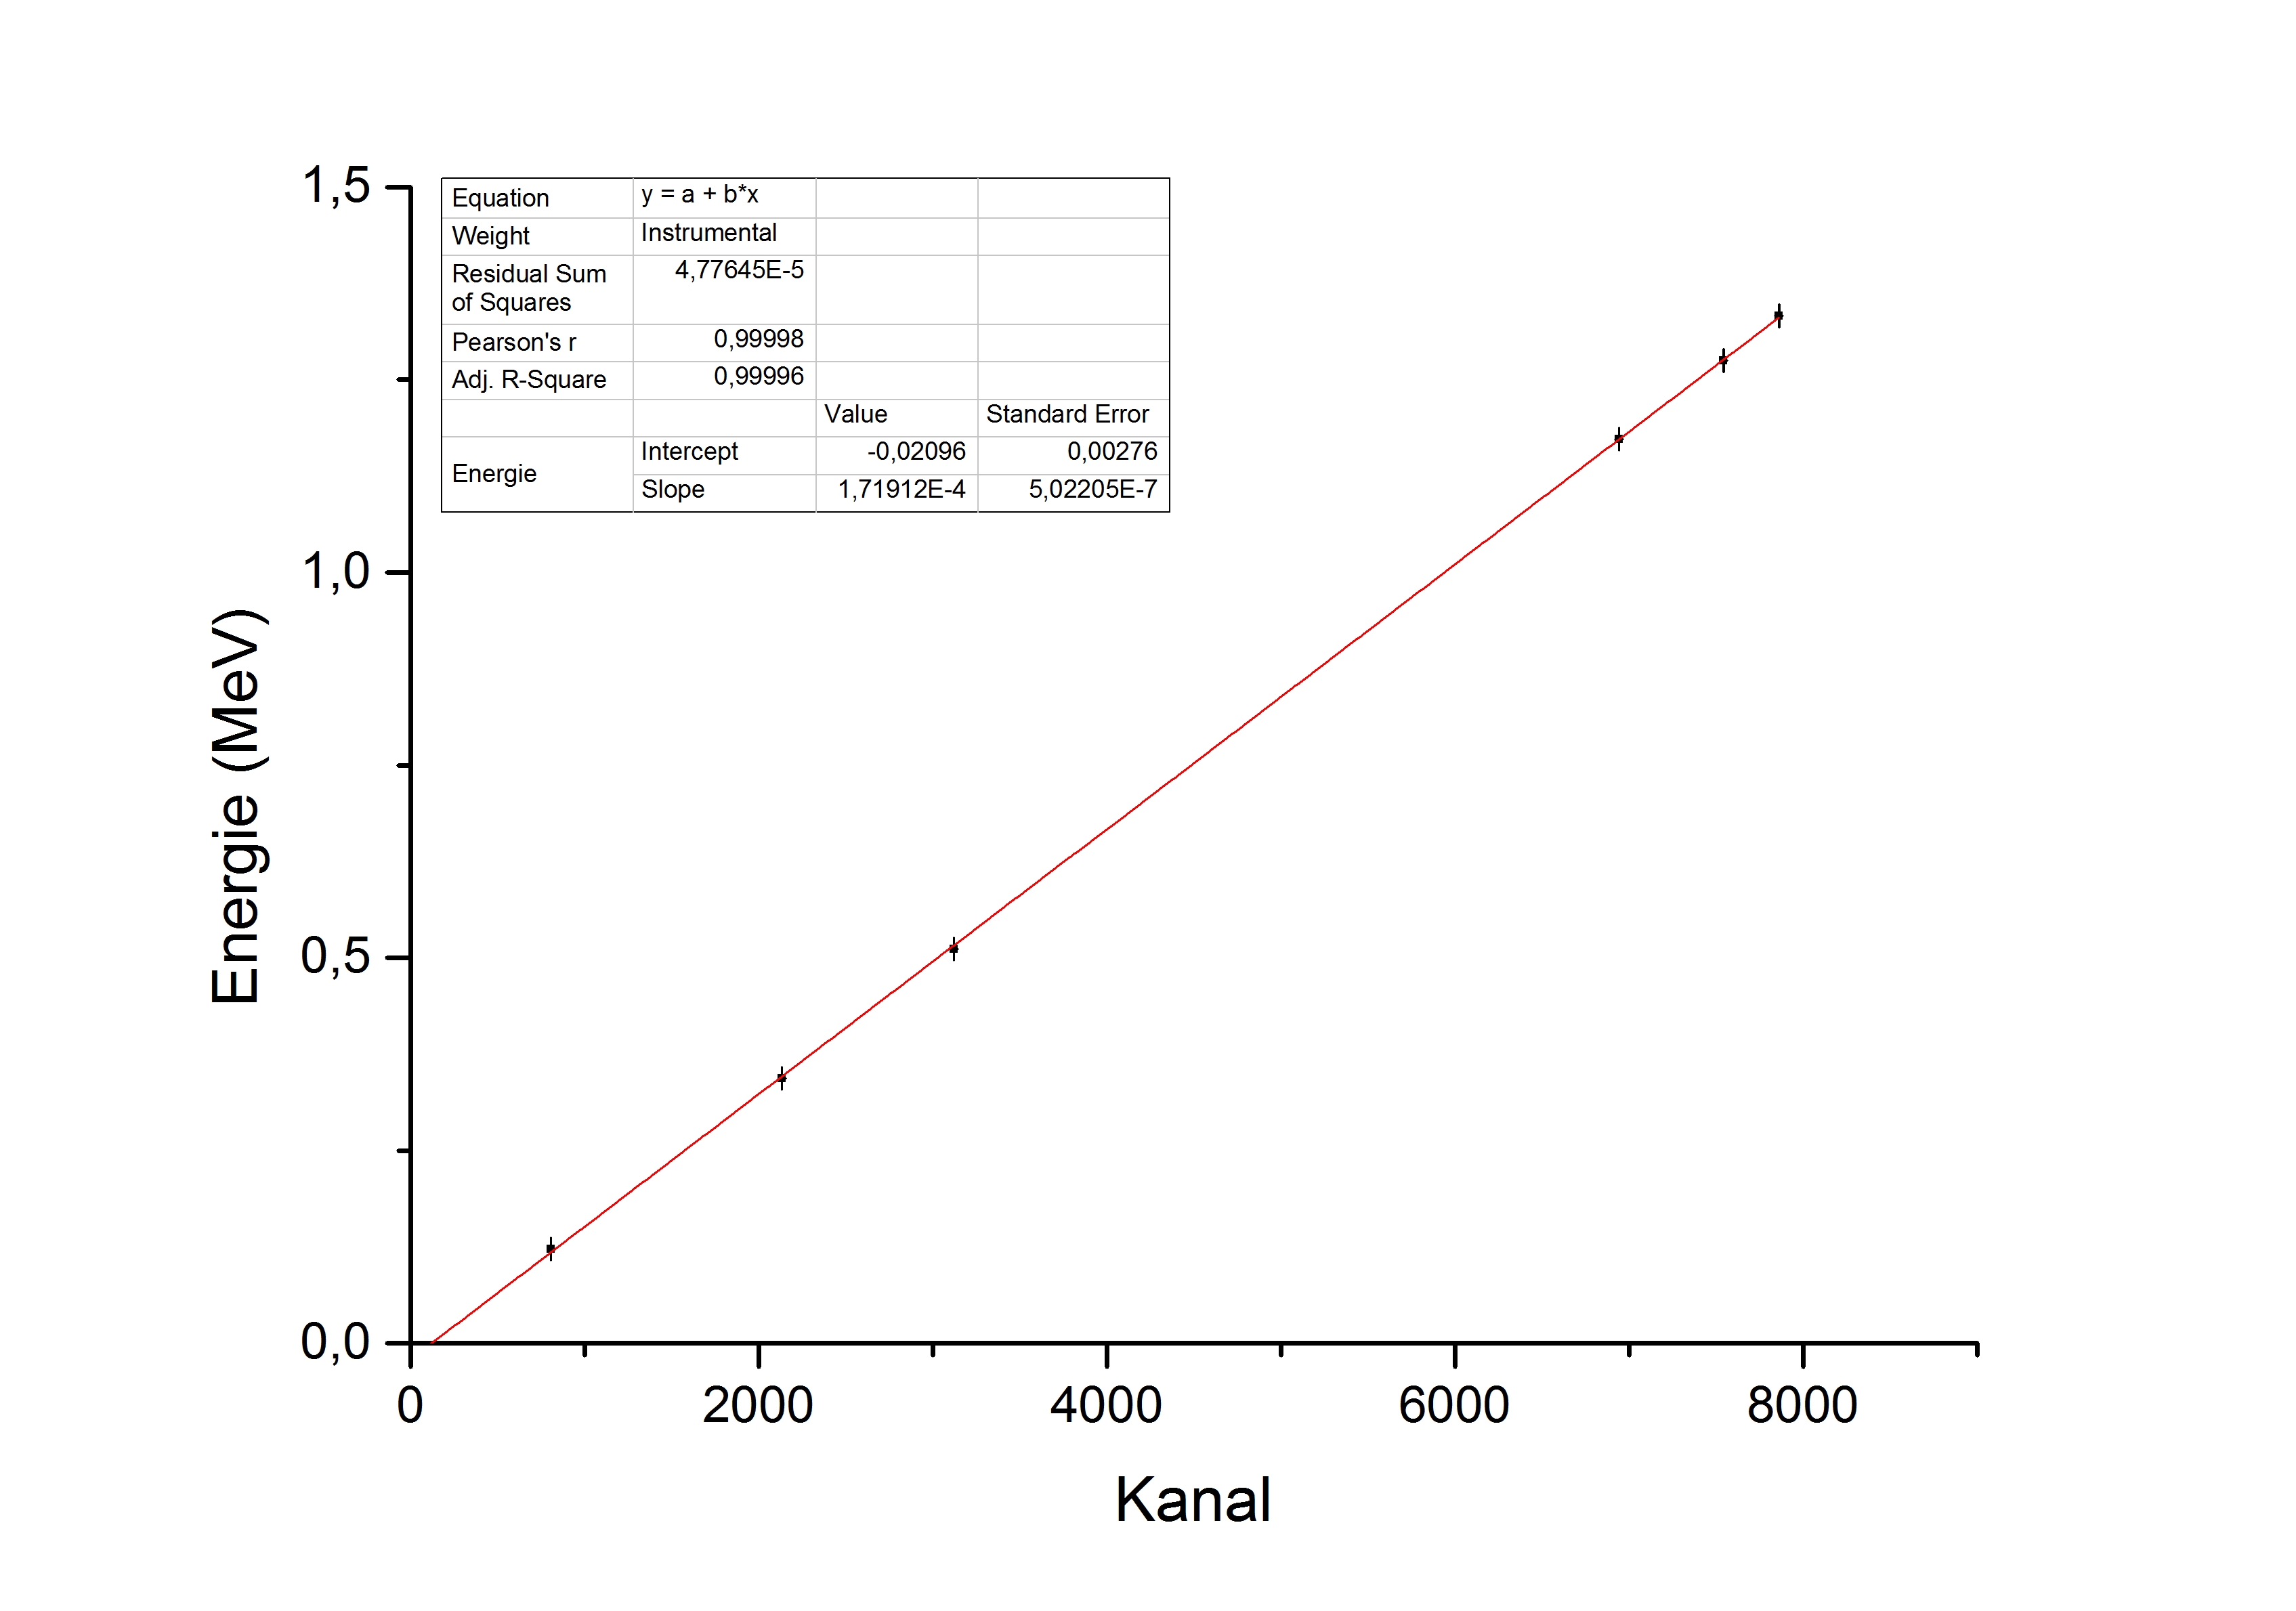
\includegraphics[scale=0.6]{Bilder/linfit}
  \caption{Linearer Fit}
  \end{center}
  \end{figure}
  Das korrigierte Bestimmtheitsmaß ('Adj. $R^{2}$) beträgt 0,99996 und ist damit sehr nahe an 1, woraus wir schließen können, dass die Daten - wie erwartet - sehr gut von einem linearen Fit beschrieben werden können. \\
  Als Umrechnungsformel von den Kanälen auf die Energie erhalten wir 
  \[E(C)=(0,1719\pm0,0005)\frac{keV}{Kanal}\cdot C+(-21\pm3)keV.\]
  Dabei ist ein Offset zu beobachten, welcher allerdings sehr gering ist.
  \subsubsection{Peak im Untergrundverlauf}
  Wie bereits erwähnt, konnte in der Untergrundmessung ein Peak beobachtet werden. Dieser wurde mit einer Gausskurve gefittet. Damit ergab sich:\\
  Kanal: $(8617,9\pm1,5)$,\\
  $\chi^{2}$/ndof=1,11715,\\
  Adj. $R^{2}$=0,92012.\\
  Der niedrige Wert für $\chi^{2}/ndof$ und besonders der ziemlich hohe Wert für das korrigierte Bestimmtheitsmaß zeugen von einem guten Fit. \\
  Mithilfe der eben berechneten Umrechnungsmethode kann die Energie des Untergrundpeaks nun berechnet werden, wobei sich der Fehler mit Gauss'scher Fehlerfortpflanzung zu 
  \[s_{E}=\sqrt{C^{2}s_{b}^{2}+s_{a}^{2}+b^{2}s_{C}^{2}}\] 
  berechnet. Somit ergibt sich als Energie des Peaks im Untergrund $E=(1461\pm5)keV$. Dabei handelt es sich vermutlich um den Zerfall von natürlich vorkommenden $^{40}K$, welches unter Anderem in den angeregten Zustand von $^{40}Ar$ zerfällt. Bei der Abregung wird ein $\gamma$-Quant mit der Energie von 1461 keV (Quelle: [sta]) freigesetzt. Die Energie des Peaks im Untergrundspektrum entspricht dieser im Rahmen der Messungenauigkeit, was die Vermutung nahelegt. 
  \clearpage
  \subsection{Analyse des $^{228}Th$-Spektrums}
  Für $^{228}Th$ betrug die tatsächliche Messdauer ('Live time') $t_{^{228}Th}=5744 s$. Die resultierende Zählrate und deren Fehler wurde analog zu dem vorherigen Unterkapitel berechnet. Die Zählrate wurde über die Kanäle aufgetragen und Peaks mithilfe der bereits diskutierten Gaussfunktion 
  \[n(C)=y_{0}+A\cdot e^{-0,5(\frac{C-C_{peak}}{w})^{2}}\]
   gefittet. Dabei haben wir aufgrund der unterschiedlichen Amplituden der Peaks das Diagramm in vier Teile aufgespalten, um diese besser sichtbar zu machen.
  \begin{figure}[h]
  \begin{center}
  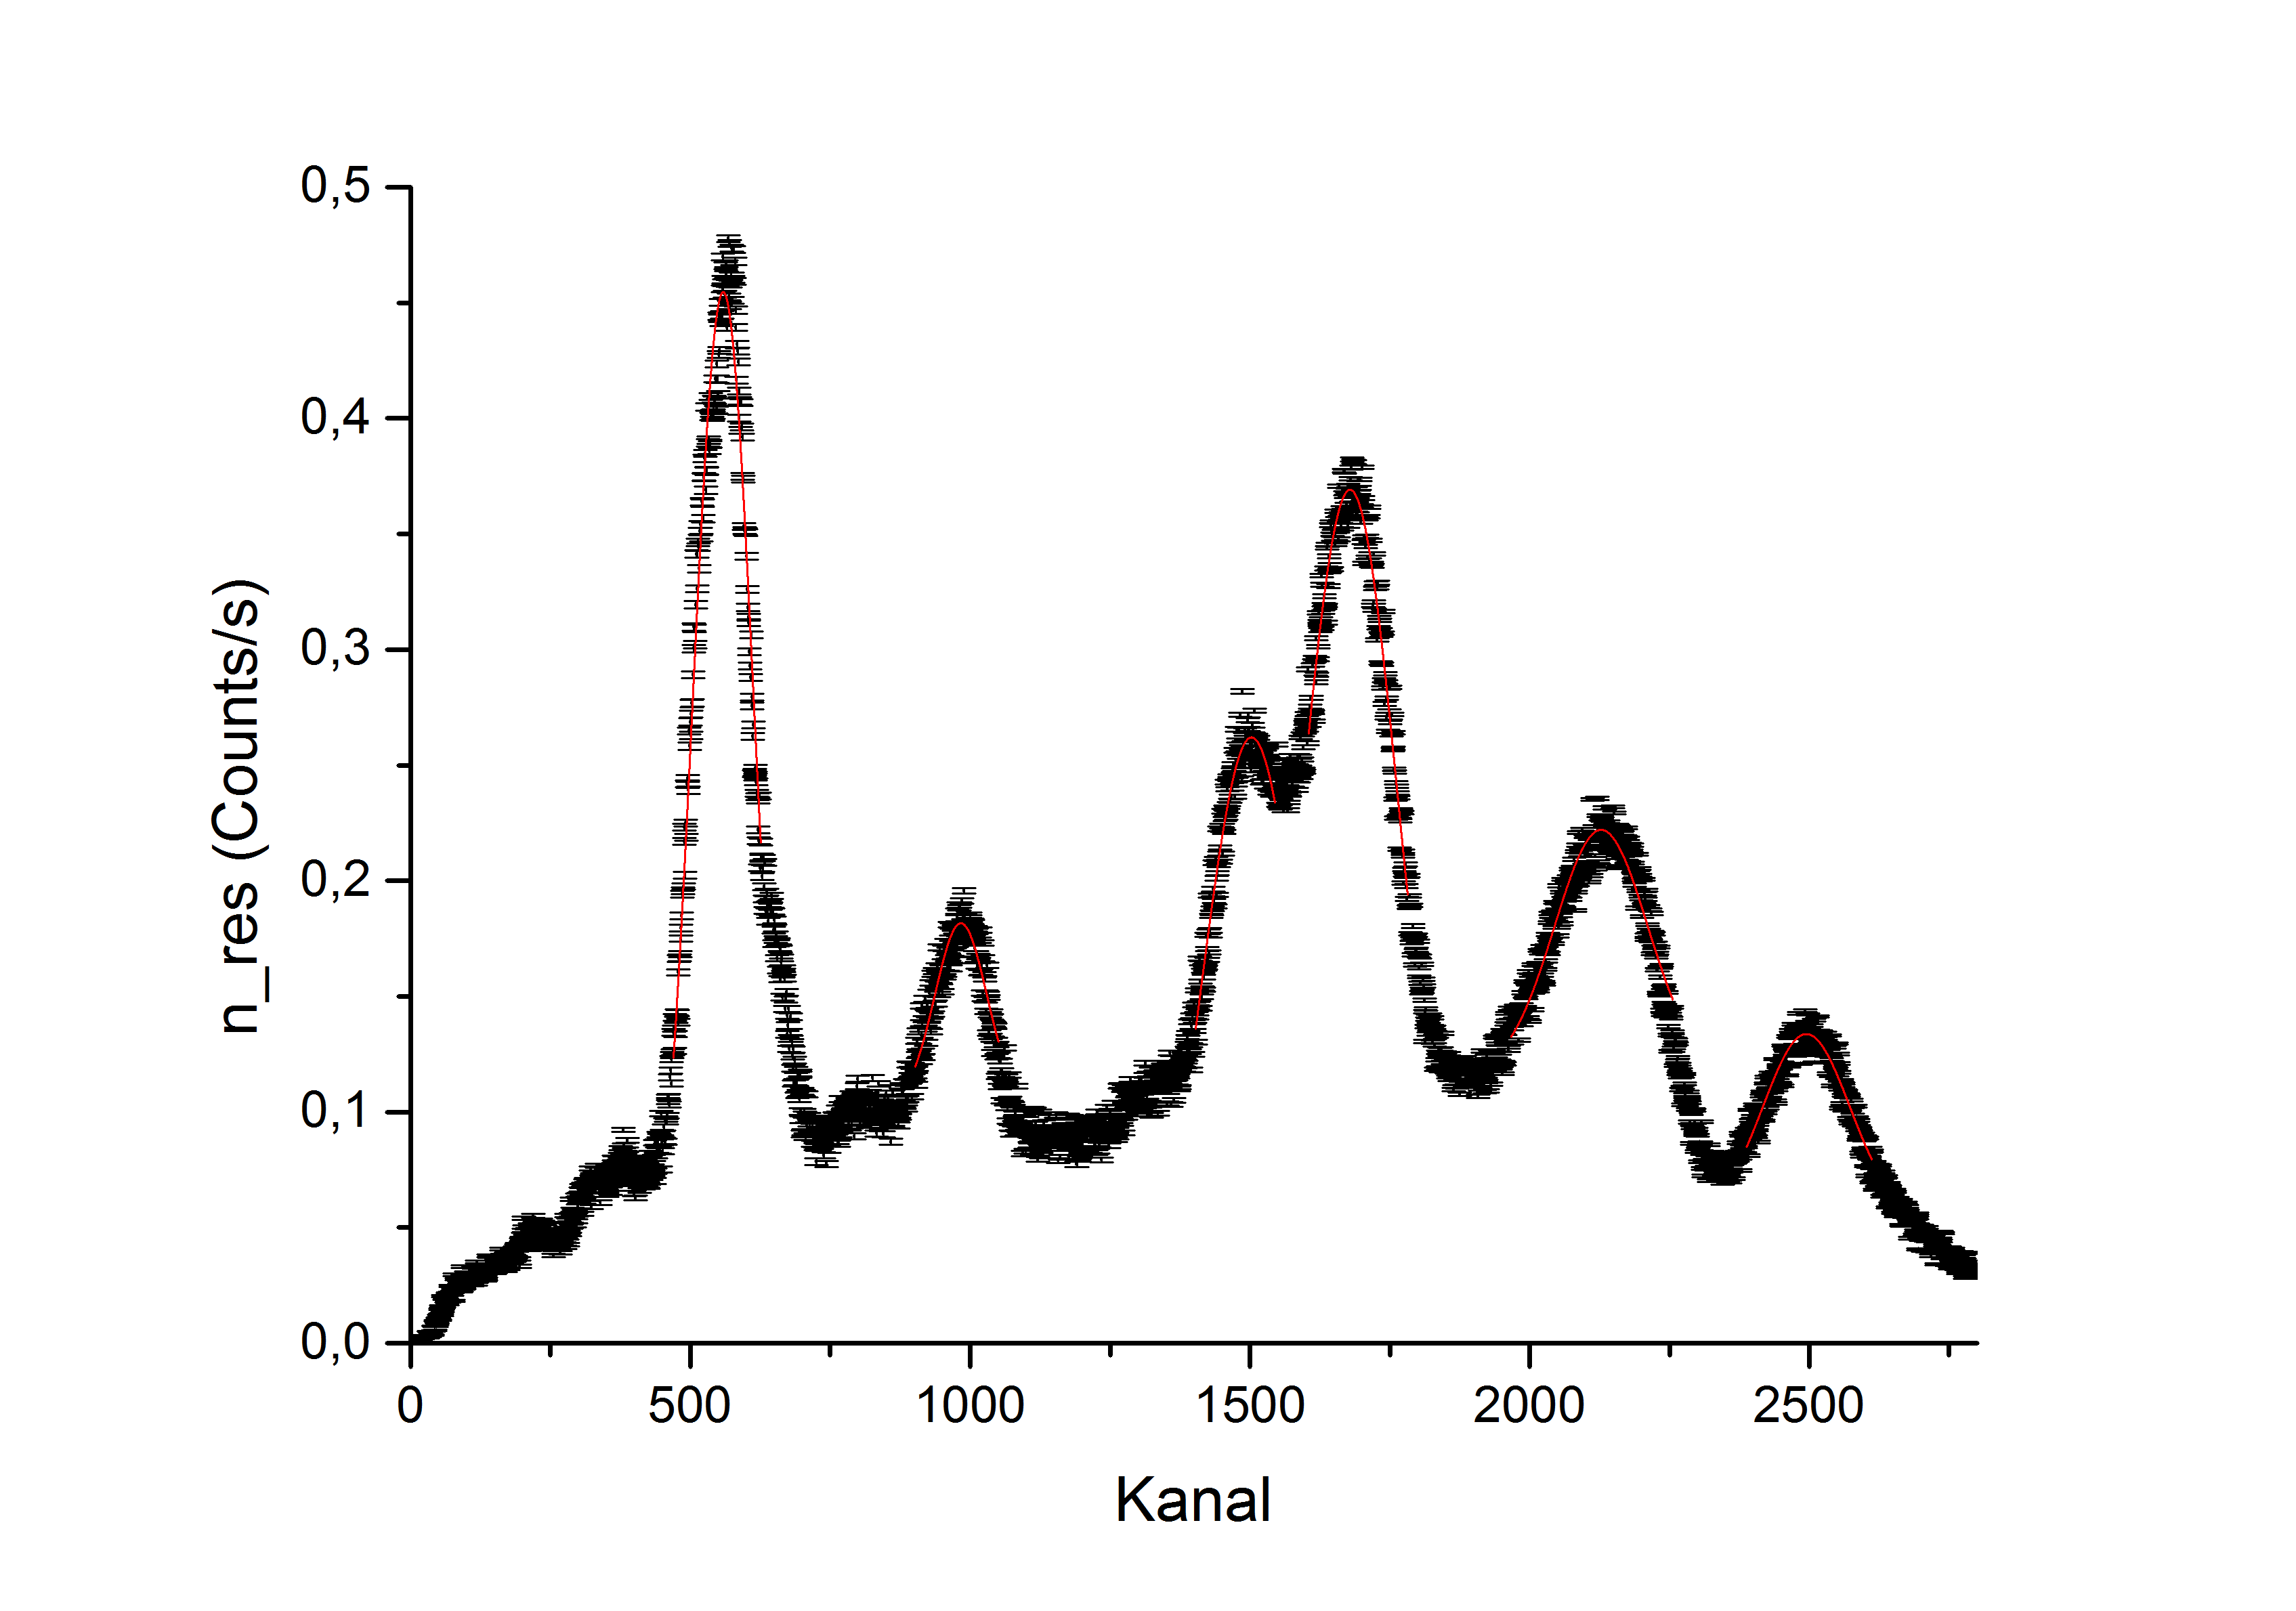
\includegraphics[scale=0.6]{Bilder/peaks1}
  \caption{Erster Teil des Thoriumspektrums}
  \end{center}
  \end{figure}
  \begin{figure}[h]
    \begin{center}
    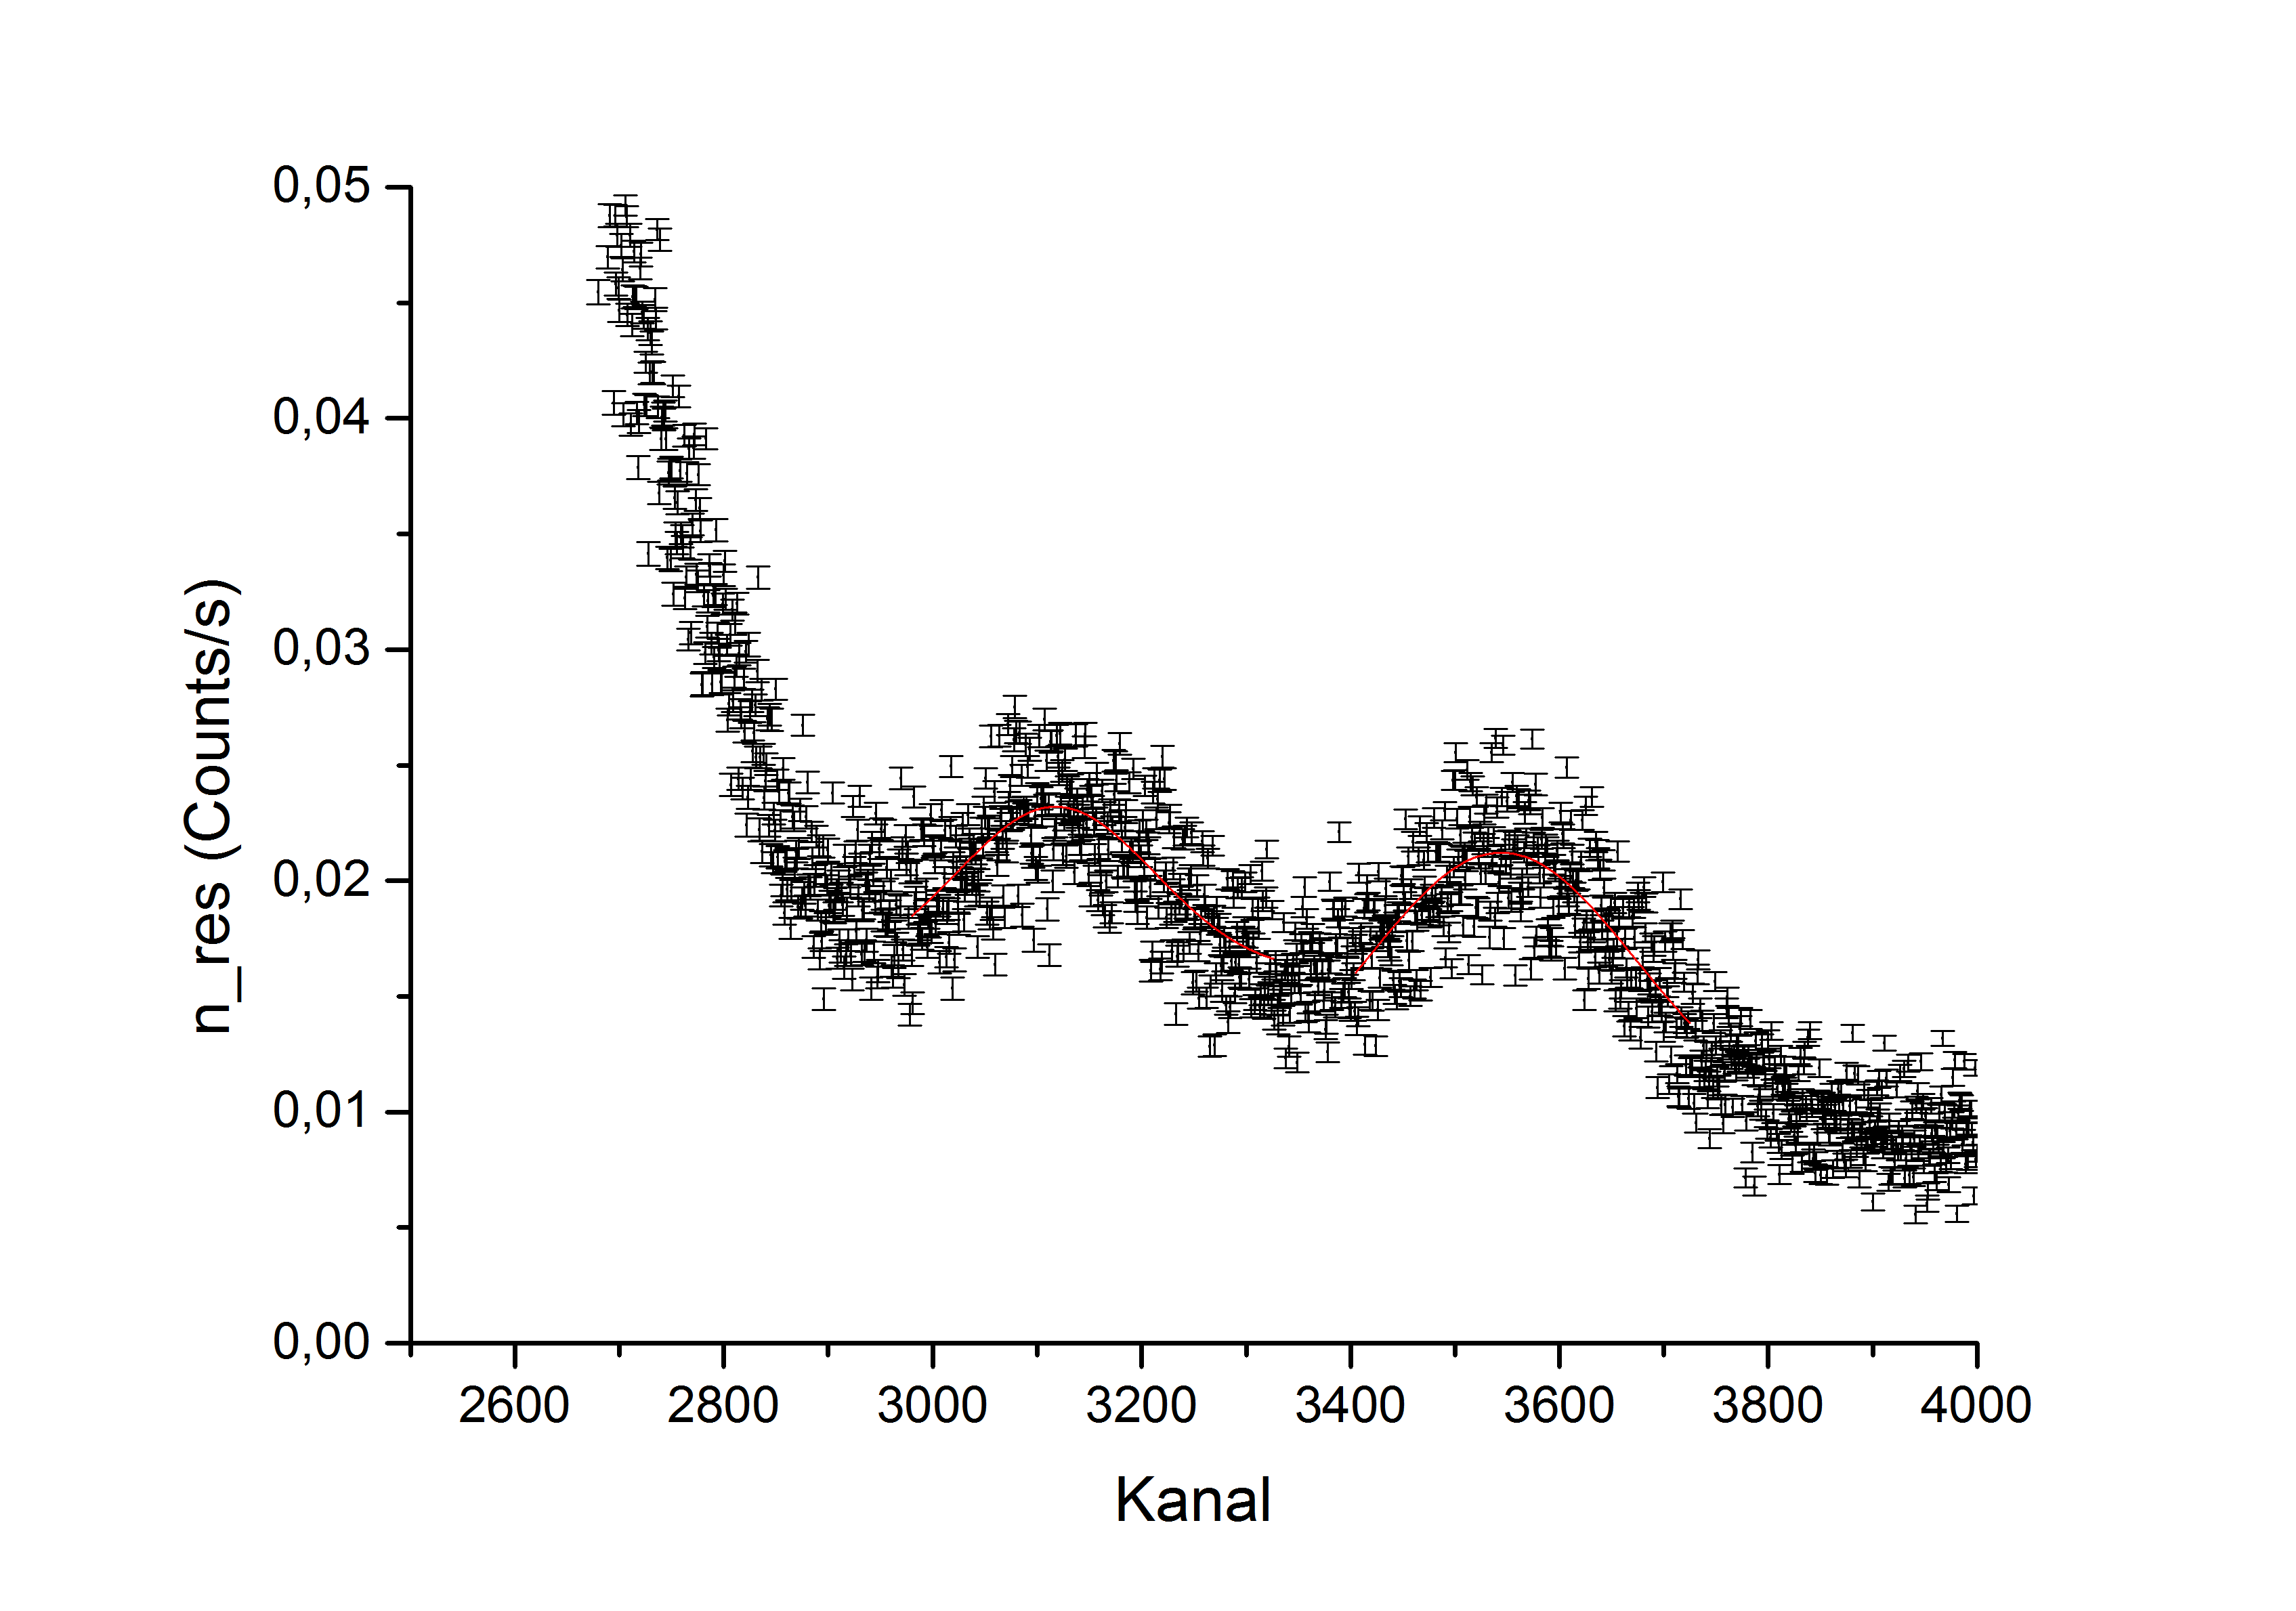
\includegraphics[scale=0.6]{Bilder/peaks2}
    \caption{Zweiter Teil des Thoriumspektrums}
    \end{center}
    \end{figure}
    \begin{figure}[h]
      \begin{center}
      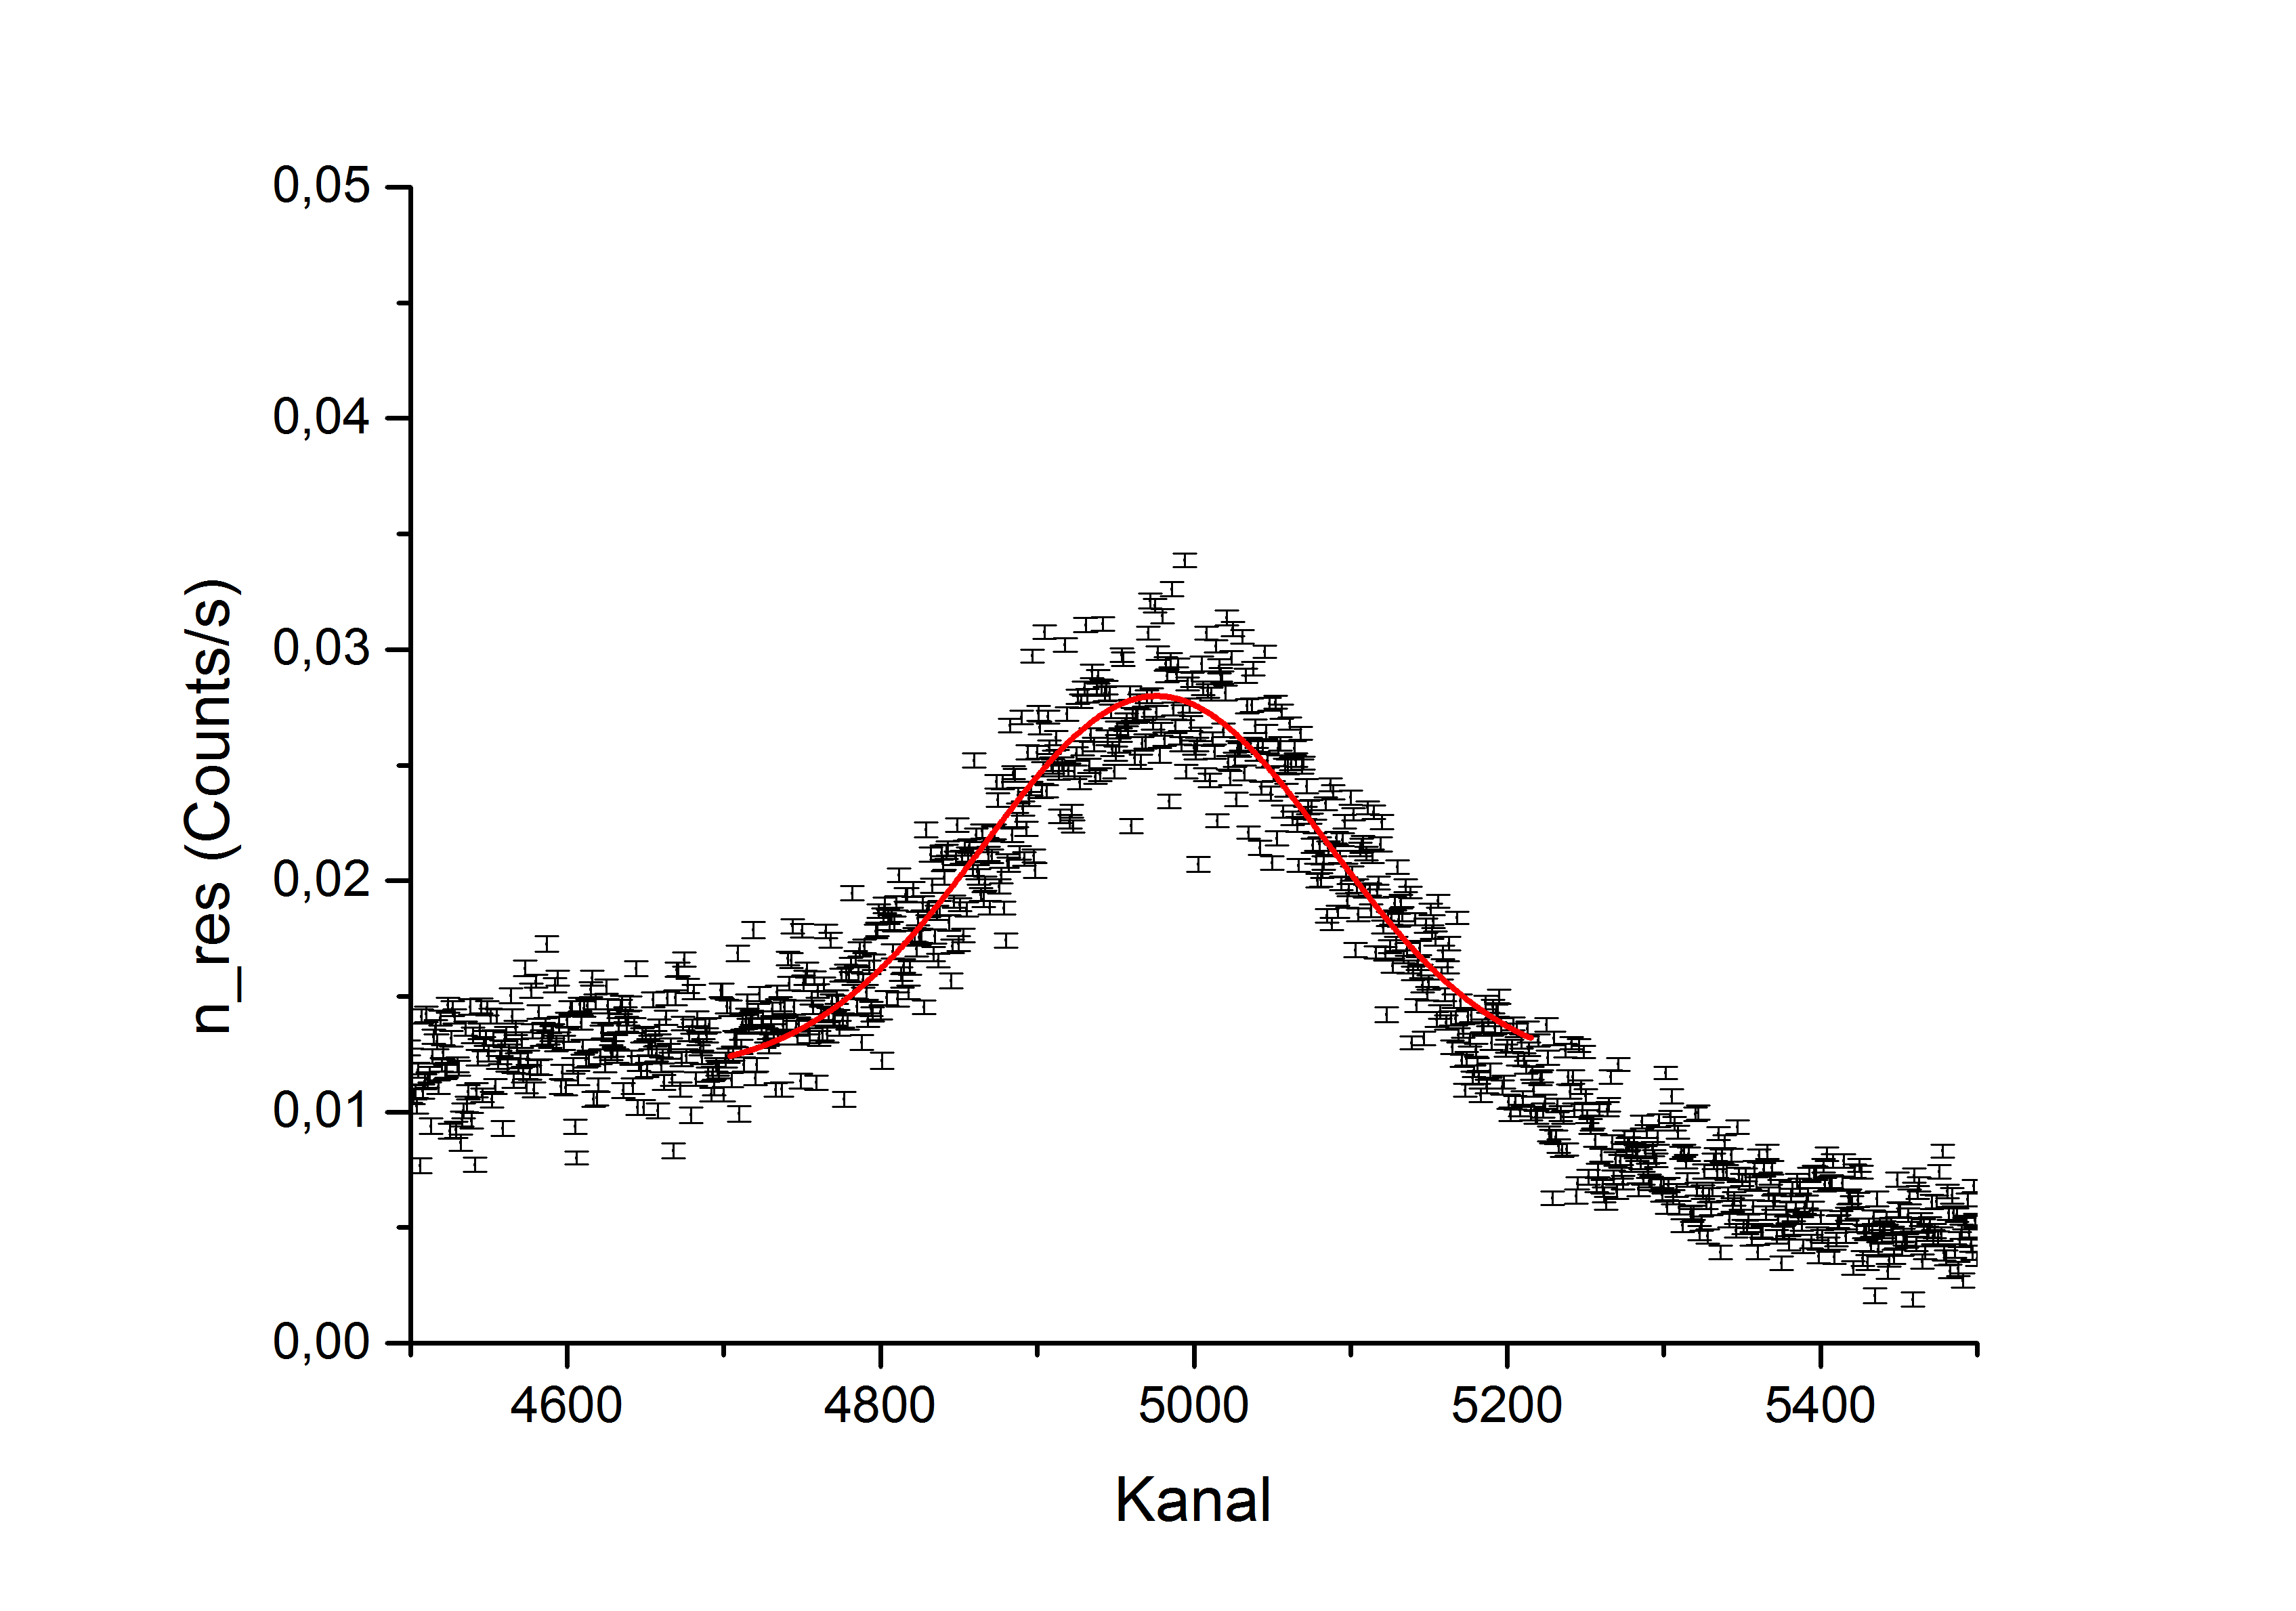
\includegraphics[scale=0.6]{Bilder/peaks4}
      \caption{Dritter Teil des Thoriumspektrums}
      \end{center}
      \end{figure}
      \begin{figure}[h]
        \begin{center}
        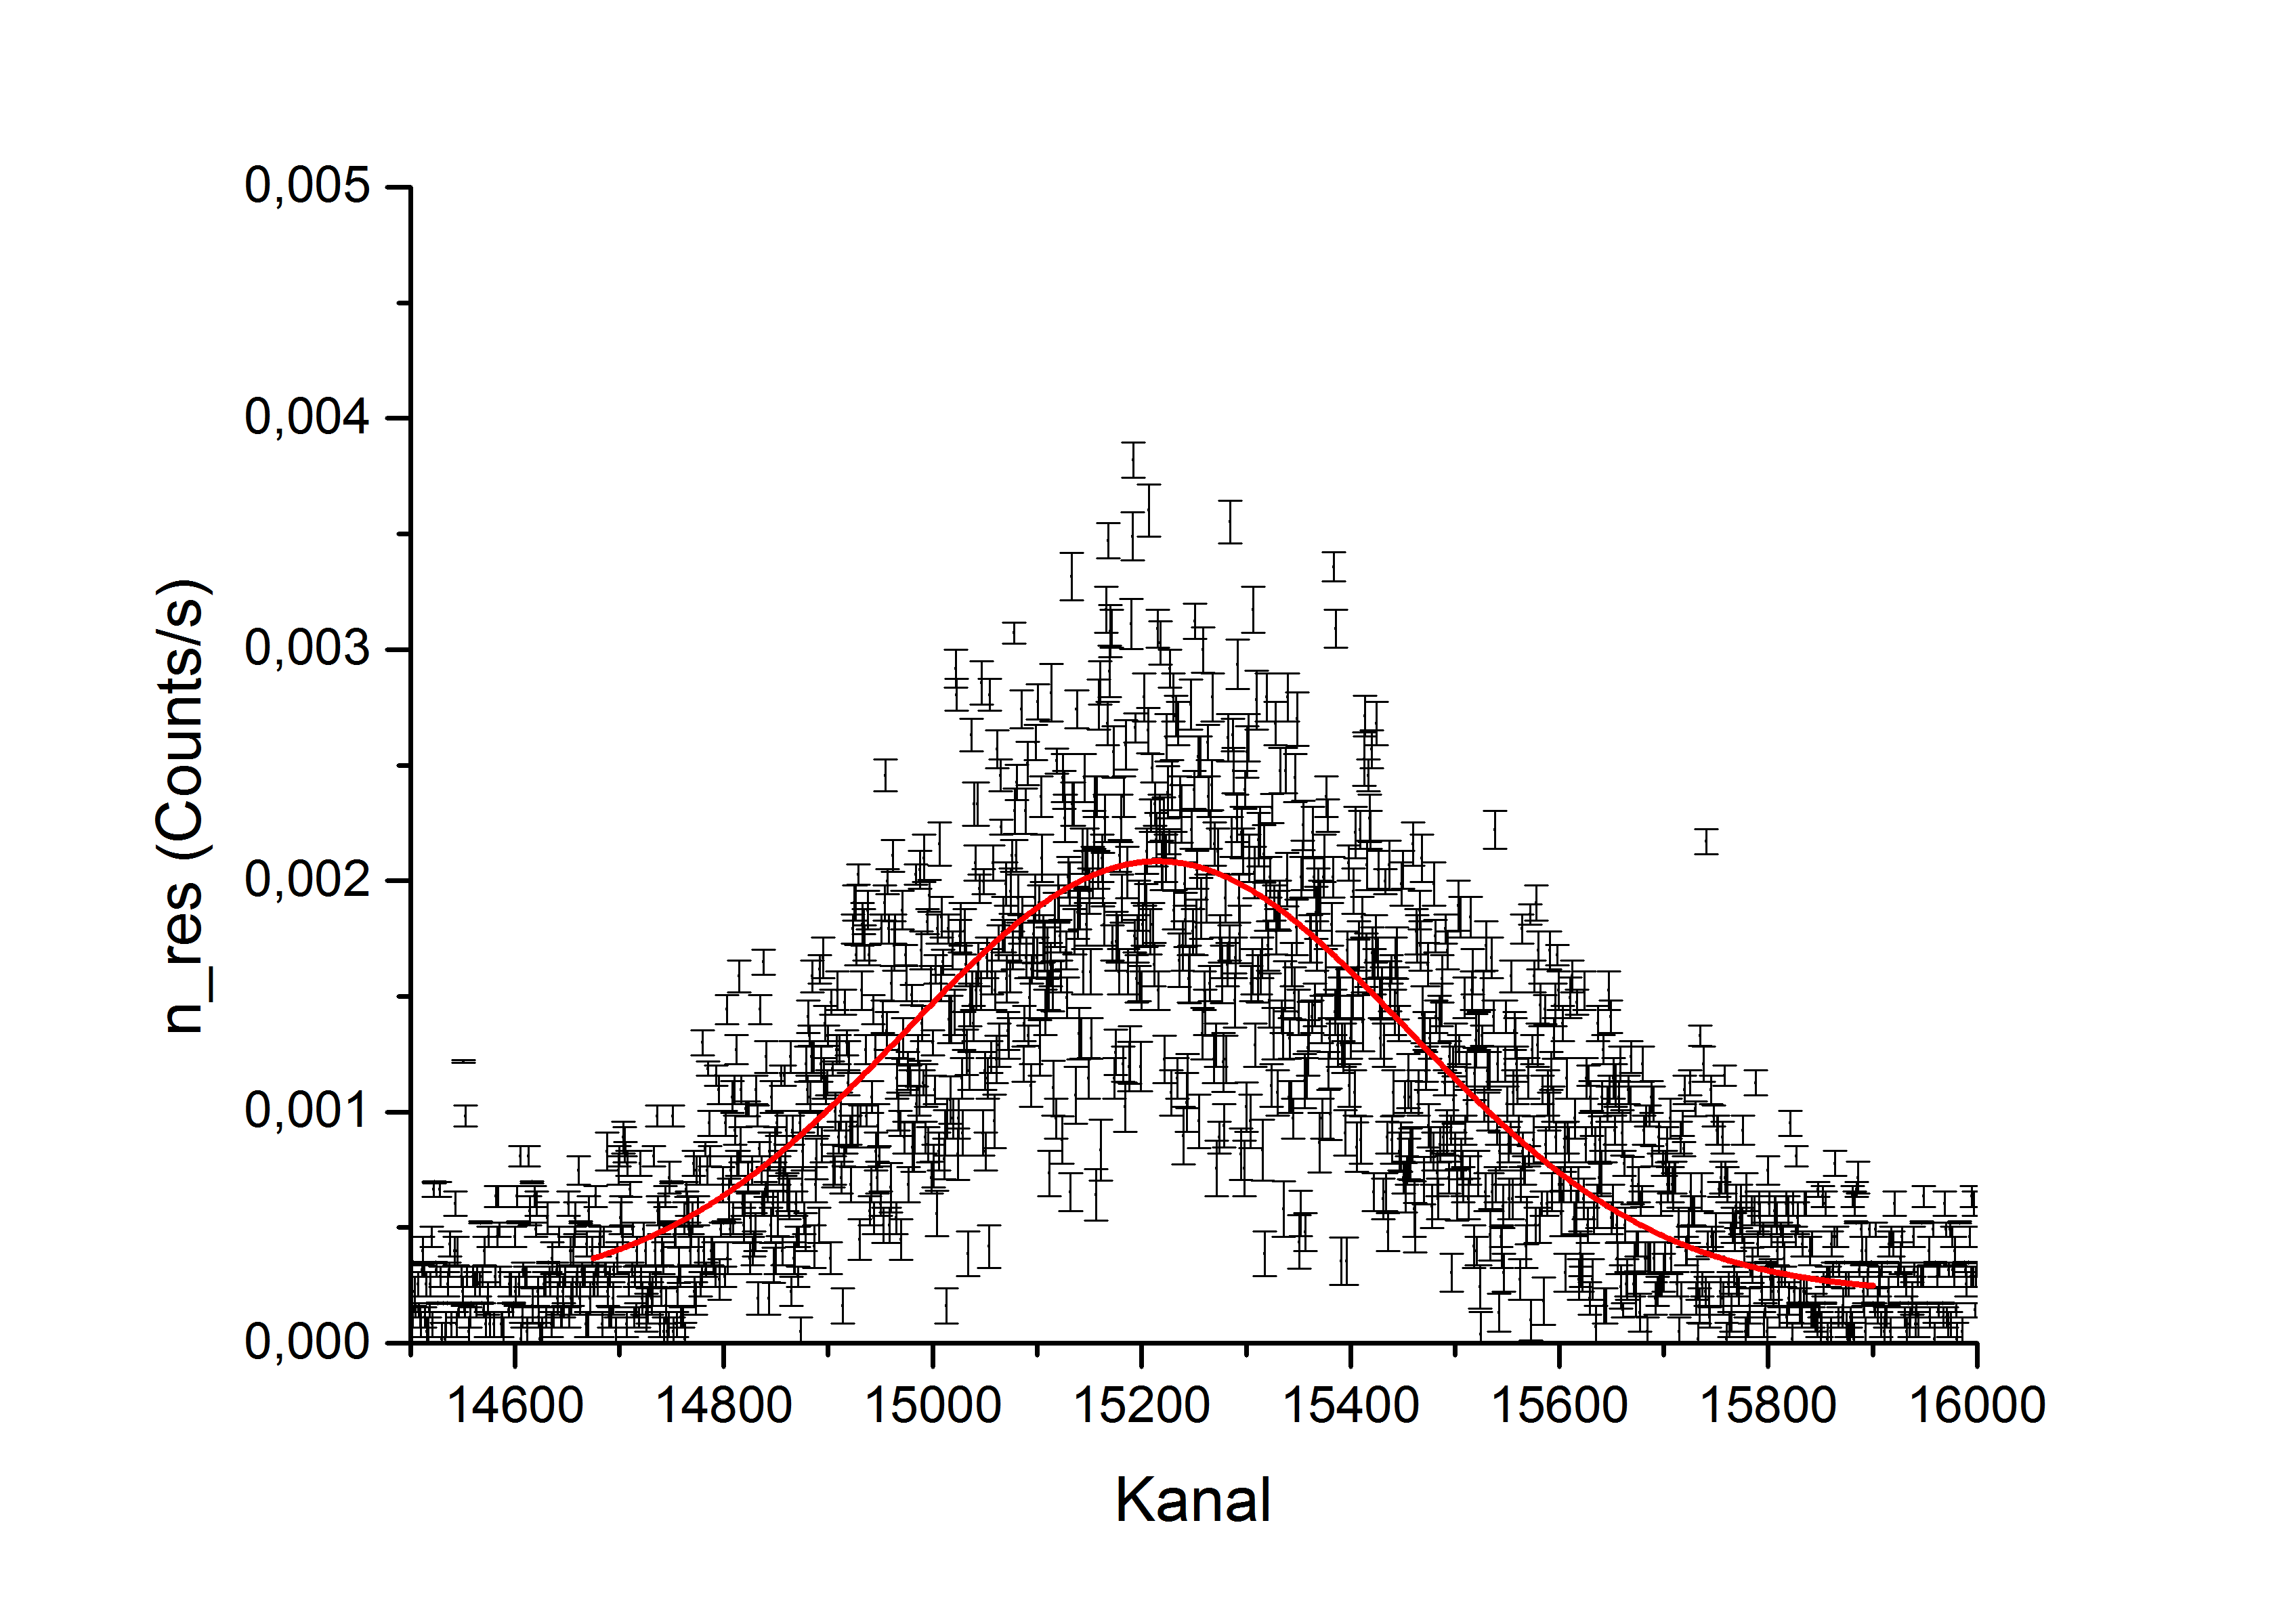
\includegraphics[scale=0.6]{Bilder/peaks3}
        \caption{Vierter Teil des Thoriumspektrums}
        \end{center}
        \end{figure}
        \clearpage
Wir erhielten 10 Peaks, für welche folgendes gilt:
\begin{table}[htbp]
\begin{center}
\caption{}
\begin{tabular}{|l|l|l|r|r|}
\hline
Kanal $C_{peak}$ & $y_{0}$ & A & \multicolumn{1}{l|}{$\chi^{2}/ndof$} & \multicolumn{1}{l|}{Adj. $R^{2}$} \\ \hline
$559,0\pm0,4$ & $0,00\pm0,03$ & $0,45\pm0,02$ & 130,44677 & 0,97255 \\ \hline
$983,8\pm0,7$ & $0,103\pm0,008$ & $0,079\pm0,008$ & 31,95607 & 0,88299 \\ \hline
$1502,9\pm0,9$ & $-0,01\pm0,05$ & $0,27\pm0,05$ & 57,0133 & 0,96581 \\ \hline
$1678,9\pm0,4$ & $0,02\pm0,04$ & $0,35\pm0,04$ & 109,08438 & 0,97422 \\ \hline
$2127,9\pm0,8$ & $0,116\pm0,005$ & $0,106\pm0,005$ & 144,6354 & 0,92679 \\ \hline
$2494,7\pm0,7$ & $0,053\pm0,008$ & $0,080\pm0,008$ & 94,91983 & 0,91688 \\ \hline
$3118\pm4$ & $0,0160\pm0,0008$ & $0,0072\pm0,0007$ & 24,06606 & 0,4671 \\ \hline
$3544\pm3$ & $0,009\pm0,004$ & $0,012\pm0,004$ & 27,91625 & 0,474 \\ \hline
$4976,3\pm1,4$ & $0,0117\pm0,0004$ & $0,0163\pm0,0004$ & 48,17991 & 0,86531 \\ \hline
$15215\pm4$ & $0,000216\pm0,000012$ & $0,00187\pm0,00004$ & 58,14617 & 0,71729 \\ \hline
\end{tabular}
\label{}
\end{center}
\end{table}
Dabei ist klar zu erkennen, dass für die hohen Peaks (bis Kanal $2494,7\pm0,7$) die Fits deutlich besser sind als für die restlichen Peaks. Die Werte für das korrigierte Bestimmtheitsmaß sind hier im Bereich von 0,9 und höher. Für die beiden Peaks bei den Kanälen $3118\pm4$ und $3544\pm3$ gilt $Adj. R^{2}<0,5$, was daran liegt, dass die Peaks räumlich sehr nahe aneinander liegen und die Zählrate niedrig ist, weshalb die Ungenauigkeiten groß werden. Die Fits für die restlichen beiden Peaks sind besser, allerdings auch nicht so gut, was daran liegt, dass die Zählrate deutlich geringer ist und damit statistische Streuungen deutlich stärker ins Gewicht fallen.\\
~\\
Auf die Peaks nehmen wir nunmehr als Peak 1-10 Bezug: Peak 1 ist dabei der Peak mit der kleinsten zugeordneten Kanalzahl, die restlichen Zahlen werden aufsteigend nach Kanalzahl zugeordnet.\\
~\\
Mithilfe der Energieeichung $E(C)=a+b\cdot C$ können nun den Peaks Energien zugeordnet werden. Diesen werden mithilfe der Zerfallsschemata in [sta] den jeweiligen verursachenden Zerfällen zugeordnet. Der Fehler auf die Energie berechnet sich mithilfe der Gauss'schen Fehlerfortpflanzung, wie bereits diskutiert, zu $s_{E}=\sqrt{s_{a}^{2}+C^{2}s_{b}^{2}+b^{2}s_{C}^{2}}$.
\clearpage
\begin{table}[h]
\begin{center}
\caption{}
\begin{tabular}{|l|l|p{10 cm}|}
\hline
 & Energie in keV & zugeordneter Zerfall (Angabe des Mutterkerns) \\ \hline
Peak 1 & $75\pm3$ & Aufgrund der hohen Intensität vermutlich Th-228 (84,4 keV). \\ \hline
Peak 2 & $148\pm3$ & Vermutlich Überlagerung der Peaks mit 131,6 keV bzw. 166,1 keV von Th-228: Getrenntes Auflösen nicht möglich. \\ \hline
Peak 3 & $237\pm3$ &  Überlagerung von Ra-224 (241,0 keV) und Pb-212 (238,6 keV) \\ \hline
Peak 4 & $268\pm3$ & Tl-208 (277,4 keV)\\ \hline
Peak 5 & $345\pm3$ & Eventuell Pb-212 (300,1 keV).  \\ \hline
Peak 6 & $408\pm3$ & Möglicherweise Bi-212 (453,0 keV). Systematische Verschiebung zu kleineren Energien durch Asymmetrie bedingt durch höheren Peak 5 möglich. \\ \hline
Peak 7 & $515\pm3$ & Tl-208 (510,8 keV). \\ \hline
Peak 8 & $588\pm3$ & Tl-208 (583,2 keV). \\ \hline
Peak 9 & $835\pm4$ & Möglicherweise Po-212 (804,9  keV). \\ \hline
Peak 10 & $2595\pm8$ & Überlagerung von Tl-208 (2614,5 keV) und Po-208 (2610,0 keV) mit geringerer Intensität. \\ \hline
\end{tabular}
\end{center}
\label{}
\end{table}
Zu den Abweichungen von den Energien der zugeordneten Zerfällen könnten Effekte wie Rückstreuung beigetragen haben. Außer den Peaks 5,6 und 9 sind aber die von uns gemessenen Werte sehr nah an den Literaturwerten. 
\subsubsection{Intensitäten}
Die Intensitäten berechnen sich aus der Höhe der Peaks. Aufgrund der Formel für die Gausskurve gilt: \[I=y_{0}+A.\] 
Der Fehler auf diese Größe berechnet sich mithilfe Gauss'scher Fehlerfortpflanzung zu 
\[s_{I}=\sqrt{s_{y_{0}}^{2}+s_{A}^{2}}.\] 
Nun muss die Charakteristik des verwendeten NaJ-Kristalls beachtet werden, welche in [ver] gegeben ist, um die Werte anzupassen. Die Werte für die Photopeak-Effizienz P haben wir aus dem Graphen abgelesen, der Fehler auf diesen Wert kommt nicht nur durch den Fehler der Energie zustande, sondern wird dominiert durch unseren Ablesefehler. Die angepasste Intensität berechnet sich dann zu \[I_{res}=\frac{1}{P}\cdot I,\]
der Fehler mittels Gauss'scher Fehlerfortpflanzung zu 
\[s_{I_{res}}=\frac{I}{P}\cdot\sqrt{\left(\frac{s_{I}}{I}\right)^{2}+\left(\frac{s_{P}}{P}\right)^{2}}.\]
\clearpage
Somit erhalten wir:
\begin{table}[htbp]
\begin{center}
\caption{}
\begin{tabular}{|l|l|l|l|}
\hline
 & Intensität I in Counts/s & Effizienz P & $I_{res}$ in Counts/s \\ \hline
Peak 1 & $0,45\pm0,04$ & $1,00\pm0,01$ & $0,45\pm0,04$ \\ \hline
Peak 2 & $0,182\pm0,011$ & $0,97\pm0,02$ & $0,187\pm0,012$ \\ \hline
Peak 3 & $0,26\pm0,07$ & $0,90\pm0,02$ & $0,29\pm0,07$ \\ \hline
Peak 4 & $0,37\pm0,05$ & $0,86\pm0,02$ & $0,43\pm0,06$ \\ \hline
Peak 5 & $0,222\pm0,007$ & $0,76\pm0,02$ & $0,292\pm0,012$ \\ \hline
Peak 6 & $0,134\pm0,012$ & $0,71\pm0,02$ & $0,188\pm0,017$ \\ \hline
Peak 7 & $0,0232\pm0,0011$ & $0,59\pm0,02$ & $0,039\pm0,002$ \\ \hline
Peak 8 & $0,021\pm0,013$ & $0,56\pm0,02$ & $0,04\pm0,02$ \\ \hline
Peak 9 & $0,0280\pm0,0006$ & $0,41\pm0,02$ & $0,068\pm0,004$ \\ \hline
Peak 10 & $0,00209\pm0,00004$ & $0,14\pm0,02$ & $0,015\pm0,002$ \\ \hline
\end{tabular}
\end{center}
\label{}
\end{table}
Da in [sta] nur relative Intensitäten gegeben sind, muss nun noch eine Normierung auf 100 erfolgen: Dazu werden die resultierenden Intensitäten von Peak i, $I_{res_{i}}$, durch $I_{res_{1}}$ von Peak 1 geteilt, da diese den höchsten Wert vorweist und das Ergebnis mit 100 multipliziert. \[I_{norm_{i}}=\frac{I_{res_{i}}}{I_{res_{1}}}\cdot 100.\] 
Der Fehler wird auch einfach durch $I_{res_{1}}$ geteilt und mit 100 multipliziert. Die so erhaltenen relativen Intensitäten werden dann mit den Literaturwerten aus [sta] verglichen.
\begin{table}[htbp]
\begin{center}
\caption{}
\begin{tabular}{|l|l|r|}
\hline
 & $I_{norm}$ & \multicolumn{1}{l|}{Literaturwert} \\ \hline
Peak 1 & $100\pm8$ & 100 \\ \hline
Peak 2 & $41\pm3$ & \multicolumn{1}{l|}{10,7 bzw. 8,49} \\ \hline
Peak 3 & $64\pm16$ & \multicolumn{1}{l|}{10 bzw. 0,41} \\ \hline
Peak 4 & $94\pm13$ & 0,636 \\ \hline
Peak 5 & $64\pm3$ & 0,757 \\ \hline
Peak 6 & $41\pm4$ & 0,101 \\ \hline
Peak 7 & $8,7\pm0,5$ & 2,28 \\ \hline
Peak 8 & $8\pm5$ & 8,52 \\ \hline
Peak 9 & $15,0\pm0,8$ & 0,0002 \\ \hline
Peak 10 & $3,3\pm0,5$ & \multicolumn{1}{l|}{10 bzw. 0,26} \\ \hline
\end{tabular}
\end{center}
\label{}
\end{table}
~\\
Für diejenigen Peaks, welchen wir zwei mögliche Übergänge zuordneten, haben wir beide Literaturwerte aufgeführt, wobei der größere Wert (vor allem bei großen Unterschieden) der relevantere Wert ist, da es wahrscheinlich ist, dass der Übergang mit höherer Intensität detektiert wurde.
Es sprechen nur Peak 8 und Peak 1 im Rahmen der Messungenauigkeit mit dem jeweiligen Literaturwert überein. Da auf Peak 1 normiert wurde (da dies der höchste Peak war), ist dies allerdings ein Ergebnis unserer Vorgehensweise.\\
Für die anderen Peaks sind erhebliche Diskrepanzen zwischen errechnetem Wert und Literaturwert zu beobachten. Dies kann darauf hinweisen, dass falsche Zuordnungen aufgrund der Energien erfolgten. Es ist aber auch möglich, dass zu wenige Counts für Peak 1 und Peak 10 bzw. zu viele für die übrigen Peaks (außer Peak 8) gemessen wurden.
